%**********
% Preamble
%**********
\documentclass[11pt]{report}

% Set packages to be used (most should be included in your LaTeX installation; the rest are locally defined)
\usepackage{amsmath,amsfonts,amsthm,../styles/commands,graphicx,../styles/project}
% amsmath      : Provides enhanced functionality for mathematical formulas
%                ftp://ftp.ams.org/ams/doc/amsmath/amsldoc.pdf
% amsfonts     : Provides additional mathematical fonts
%                ftp://ftp.ams.org/pub/tex/doc/amsfonts/amsfndoc.pdf
% amsthm       : Provides enhanced commands for theorem-like environments
%                ftp://ftp.ams.org/ams/doc/amscls/amsthdoc.pdf
% commands     : Provides short-cut commands (locally defined)
% graphicx     : Provides enhanced support for graphics
%                http://en.wikibooks.org/wiki/LaTeX/Importing_Graphics#The_graphicx_package
% project      : Provides project format (locally defined)
% Other packages you may want to consider:
% amssymb, hyperref, longtable, natbib, rotating

%**********
% Document
%**********
\begin{document}

%************
% Title page
%************

\title {A survey on some nonlinear programming algorithms}
\author{Xi He}

%*************
% Figure List
%*************
%\figurespagefalse % Uncomment if you do not have figures

%************
% Table List
%************
%\tablespagefalse % Uncomment if you do not have tables

%*********
% Preface
%*********
\preface
%*********
% Chapter
%*********
\chapter{Introduction}

This project concerns the practical implementation of several classical optimization algorithms in the context of unconstrained nonlinear problems. By choosing proper parameter set and delicate implementation, we intend to achieve economy of computation or the solution of such problems. With respect to several test problems, we compare the various performance of each algorithms with different parameters setup. It also might be a reasonable instruction on deciding which algorithm should be applied when faced a new problem.

At the first part of this project, we study several algorithms on solving unconstrained nonlinear optimization problems, such as steepest descent method, newton method and BFGS method with two kinds of linear search strategy: backtrack line search method and wolfe line search method. Trust region method is also argued with two similar approaches to solve trust region subproblem: conjugate gradient method and conjugate gradient method with SR1 Hessian matrix update method. Throughout the introduction of each algorithm, we also list convergence and complexity issues, however, one should note that we state some correct conclusions without rigorous proof.

In the latter part of this project, some detailed implementation concerns are discussed with respect to different problems and algorithms, including practical parameter set choosing, tricks on attaining economy computation and also some difficulties with respect to implementation. Results on numerical experiment are shown to clearly compare the performance of each algorithm with different parameters on each problem. Also, some analysis of the numerical result are presented.

The structure of this project report is as follows. Chapter 2 includes relevant background on unconstrained optimization problems which forms the basis of the discussions in later chapters. In Chapter 3, after showing the very basic two descent directions we used in implementation, we discuss two kinds of linear search strategy. And then we present two kinds of quasi-newton method and show the global convergence results when applying the two line search method mentioned before. We introduce in Chapter 4 about trust region algorithms and conjugate gradient method with is proposed by solving the trust region subproblems. SR1 update which is stated in Chapter 3 will be reconsidered as a approach to solving trust region subproblem when combining with conjugate gradient method. Finally, in Chapter 5, we present, analyze and provide numerical results with respect to the algorithms we discuss in above chapters on some test problems. Brief summary of this project and some general conclusion will be stated in the Chapter 6. 

In this report, we use the following notation. Let $f(x)$ be original nonlinear, smooth and differentiable objective function we want to minimize and $x$ be decision variables. We also denote gradient function of $f(x)$ by $g(x)=\nabla f(x)$ and denote $H(x)=\nabla^2 f(x)$ and $B(x)$ by the Hessian and approximation Hessian matrix of $f(x)$ at point $x$. With respect to algorithms, we use $d(x)$ to be an acceptable descent directions at point $x$ and $\alpha(x)$ to be an acceptable step-size along $d(x)$. At the last, $H\succ(\succeq) 0$ represents that the matrix is (semi) positive definite. 
% The introduction should include a description of the project and a summary of the contents of the report.  In particular, it should provide a high-level description of the algorithms you have implemented, the challenges that you faced, and the highlights of your numerical experiments.  The introduction should include \emph{minimal} mathematical detail, if any at all.

% The remaining chapters in this template suggest a way to format your report.  However, if you use this template, then you are not required to structure the report in the way that is outlined here.  Please feel free to change the names of chapters and/or organize your report differently.

%*********
% Chapter
%*********
\chapter{Fundamentals of Unconstrained Optimization}
We frame this report in the context of the unconstrained optimization problem
\begin{equation}
    \min_x \quad f(x),
\end{equation}

where $x\in \R^n$ is a real vector with $n\geq 1$ components $f:\R^n\rightarrow \R$ is a smooth function.

Generally, we intend to find out a global minimizer of $f$, a point where the function attains its least value in whole space. We state a formal definition as
\begin{definition}
    A point $x^*$ is a global minimizer if $f(x^*)\leq f(x)$ for all $x$.
\end{definition}

Note that it can be very difficult to find the global minimizer, since our knowledge of $f$ is usually only local. Actually, most algorithms are able to find only a local minimizer, a point that achieves the smallest value of $f$ in its neighborhood.
\begin{definition}
    A point $x^*$ is a local minimizer if there is a neighborhood $\Ncal$ of $x^*$ such that $f(x^*)\leq f(x)$ for $x\in \Ncal$.
\end{definition}

As it is shown in Figure \ref{fig:global_min}, in general case, a function $f$ may have a lot of local minimizers but just one global minimizer. Most algorithms is sensitive on the initial point we chose, which means, by choosing different initial point to run those algorithms, we may get different local minimizer.

\begin{figure}[htpb]
    \centering
    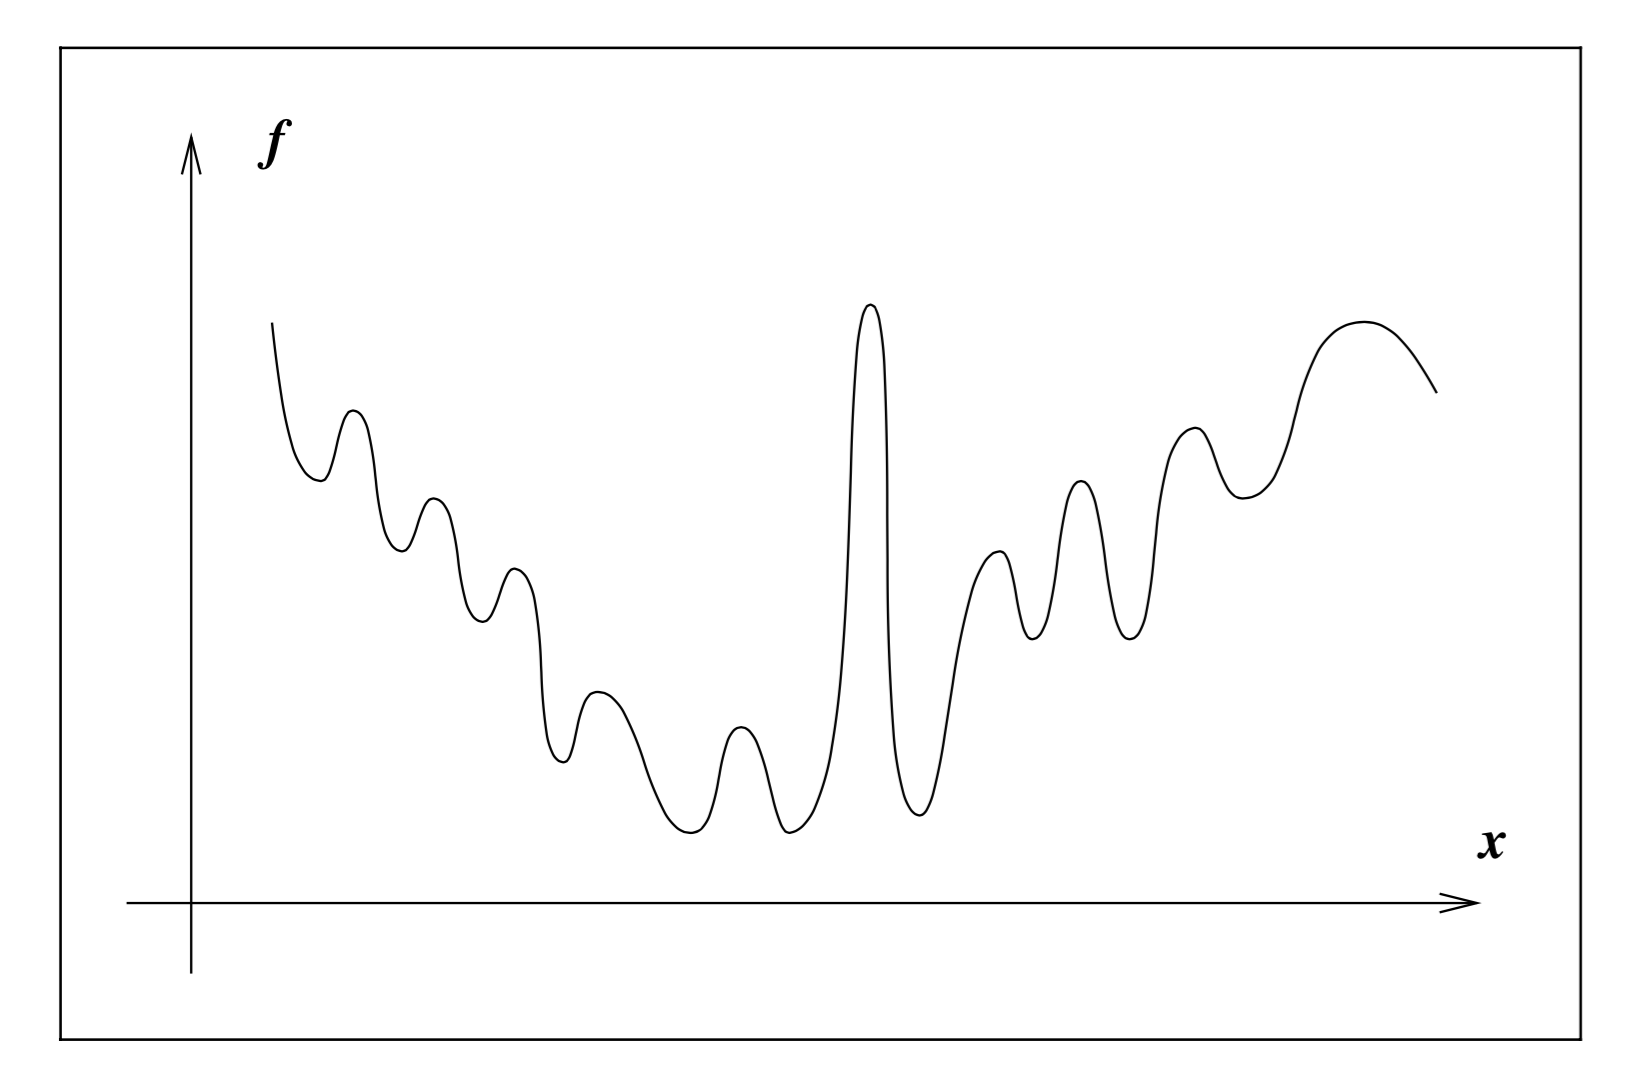
\includegraphics[width=0.95\textwidth]{../images/global_min}
    \caption{Global minimum and Local minimum}
    \label{fig:global_min}
\end{figure}

A special case we should concern is that of convex functions, every local minimizer is also a global minimizer. We state formal definition of convex as following
\begin{definition}
    A function $f: \R^n \rightarrow \R$ is convex if for all $\{x_1,x_2\}\in \R^n$ and $\alpha\in [0,1]$ we have
    \begin{equation}
        f(\alpha x_1 +(1- \alpha)x_2)\leq \alpha f(x_1) +(1- \alpha)f(x_2).
    \end{equation}
\end{definition}

Therefore, to solve a unconstrained optimization with respect to a convex objective function, we have conclusion that
\begin{theorem}
When $f$ is convex, any local minimizer $x^*$ is a global minimizer of $f$. If in addition $f$ is differentiable, then any stationary point $x^*$ is a global minimizer of $f$.
\end{theorem}

When turns to general case, i.e., objective function is not assuming to be convex but still smooth, we have following efficient and practical ways to identify local minima. To do it, we need have knowledge of the gradient $g(x^*)$ and the Hessian $H(x^*)$ of function $f$ at point $x^*$.
\begin{theorem}(First-Order Necessary Conditions)\label{thm:first_order}
    If $x^*$ is a local minimizer and $f$ is continuously differentiable in an open neighborhood of $x^*$, then $g(x^*)=0$.
\end{theorem}

We call $x^*$ a stationary point if $g(x^*)=0$. According to Theorem \ref{thm:first_order}, any local minimizer must be a stationary point. When consider Hessian matrix, we have the following conditions
\begin{theorem}(Second-Order Necessary Conditions)
If $x^*$ is a local minimizer of $f$ and $H$ is continuous in an open neighborhood of $x^*$, then $g(x^*) = 0$ and $H(x^*)$ is positive semidefinite.
\end{theorem}

Now, we state sufficient conditions, which are conditions on the derivatives of $f$ at the point $x^*$ that guarantee that $x^*$ is a local minimizer.
\begin{theorem}(Second-Order Sufficient Conditions)
Suppose that $H$ is continuous in an open neighborhood of $x^*$ and that $g(x^*) = 0$ and $H(x^*)$ is positive definite. Then $x^*$ is a strict local minimizer of $f$.
\end{theorem}

\chapter{Algorithm Descriptions I: Flexible Step Method}\label{chp: flexible}

% This chapter may discuss the algorithms that you have implemented, with comments on their similarities and differences.  For the reader's convenience, it may be useful to organize your discussion into sections, as suggested here.

% This chapter may include a citation, say to the textbook.  A citation is created in the following way: ``Please see \cite{NoceWrig06} for further details.''  The first time that you compile this template, you will most likely find that the citation appears only as a question mark and no entry is created in the Bibliography page later on.  This is because, when compiling a \LaTeX\ document with a bibliography section, you need to run \texttt{bibtex} to generate the necessary bibliography files.  (You should be able to do this easily using your \LaTeX\ IDE.)  Once this is done, then after you compile your code again, the citation should appear as a numbered reference to an entry in the Bibliography section of the report.  (Note that you may need to run \texttt{bibtex} and compile your code a few times each in order for everything to sync correctly.)

%*********
% Section
%*********

\section{Steepest Descent and Newton method}

\section{Line Search Methods}

\section{Quasi-newton method}

% This section may summarize the line search methods that you have implemented.  Most likely, this will involve writing one or more equations.  You can write equations in-line, such as $Ax=b$, or you can write them as displayed equations, such as
% \bequationn
%   Ax = b
% \eequationn
% or, perhaps better yet, as
% \bequation\label{linearsystem}
%   Ax = b.
% \eequation
% Note that if you write the equation in the latter manner, then by using the \texttt{$\backslash$label} command, you can easily refer to this equation anywhere else in your document.  You refer to an equation like this: ``Equation~\eqref{linearsystem} has zero, one, or infinitely many solutions.''  If you create more equations before and/or after the one above, then \LaTeX\ will automatically renumber all of the equations so that they are in chronological order, and will update the references accordingly.  This is much easier than having to update equation number references manually, and reduces errors.

%*********
% Section
%*********
\chapter{Algorithm Descriptions II: Restricted Step Methods.}\label{chp: restricted}

\section{Trust Region Method}

\section{Conjugate Gradient Method}

\section{Trust Region Subproblem}

% This section may summarize the trust region methods that you have implemented.  This may or may not involve providing one or more figures to illustrate the methods.  An example format for a figure can be seen in the \LaTeX\ code for producing Figure~\ref{logo} below.

% \bfigure[ht]
%   \centering
%   
\includegraphics[height=1in]{../images/lehigh}
%   \caption{Lehigh University logo}
%   \label{logo}
% \efigure

% Note that it is important to provide a useful caption for the figure.  Moreover, we again provide a label so that if we want to refer to the figure anywhere else in the report, we can do so easily.

%*********
% Chapter
%*********
\chapter{Numerical Results}

This chapter contains numerical results with respect to those algorithms we discussed in Chapter \ref{chp: flexible} and \ref{chp: restricted}. 

Note that all algorithms are implemented by Matlab under Intel Core $i5$ $2.6$ GHz processor and $8$ GB memory. Throughout this chapter, with respect to each algorithm, we use $Iter.$ to represent the total number of Iter.ations it takes to meet termination conditions. If the actual $Iter.$ is greater than defined $maxiter$, we mark $Iter.$ by a slash. $Cputime$ stands for total time of a algorithms spend to find the minimizer and when the corresponding $Iter.$ is marked as a slash, $Cputime$ means time cost up to $maxiter$ iteration. We denote $xNorm$ by the norm of difference between ending point of an algorithm and the accurate minimizer. $gNorm$ represents for the norm of gradient at the ending point.

We begin by providing some general comments that may be useful for achieve a economy computation. 

We set the default parameter value as following
\begin{table}[htpb]
    \caption{Default Parameter Set}
    \label{tab:default_para}
    \begin{center}
        \begin{tabular}{l|ccccc}
        \hline
        \hline
        \textbf{i} & \textbf{maxiter} & \textbf{opttol} & \textbf{(c1ls,c2ls)}& \textbf{(c1tr,c2tr)}\\
        \hline
             \textbf{value}& $1000$&$10^{-6}$ & $(10^{-4},0.9)$ &${(0.3,0.9)}$\\
        \hline
        \hline
        \textbf{i} & \textbf{cgopttol}& \textbf{cgmaxiter}& \textbf{sr1updatetol}& \textbf{bfgsupdatetol}& \textbf{radius} \\
        \hline
         \textbf{value}& $10^{-6}$& $50$ & $10^{-6}$ & $0.2$ &$0.25$\\
        \hline
        \hline
        \end{tabular}
    \end{center}
\end{table}

By this default set, we state numerical results for all four test problems, respectively.

\textbf{(1) Rosenbrock }

Objective function: 
\begin{equation}
    f(x_1,x_2) = 100(x_2-x_1^2)^2+(1-x_1)^2.
\end{equation}

Accurate minimizer:
\begin{equation}
    (x_1,x_2) = (1,1).
\end{equation}

Numerical results with initial point $0\mathbf{e}$:
\begin{table}[htpb]
    \caption{Rosenbrock, with initial $0\mathbf{e}$}
    \label{tab:Rosenbrock_initial}
    \begin{center}
        \begin{tabular}{l|cccc}
\textbf{Rosenbrock}           &   \textbf{xNorm}     &\textbf{gNorm}     & \textbf{Iter.}&  \textbf{Cputime}   \\
\hline
steepestbacktrack   &   $1.253e+00 $&   $1.574e-01 $&   $- $&    $0.6407    $    \\
steepestwolfe       &   $1.255e+00 $&   $1.010e-01 $&   $- $&    $0.5415    $    \\
newtonbacktrack     &   $1.414e+00 $&   $9.801e-07 $&   $13   $&    $0.0660    $    \\
newtonwolfe         &   $1.414e+00 $&   $3.652e-10 $&   $14   $&    $0.0810    $    \\
trustregioncg       &   $1.414e+00 $&   $1.310e-07 $&   $42   $&    $0.0855    $    \\
sr1trustregioncg    &   $1.414e+00 $&   $3.032e-07 $&   $77   $&    $0.0822    $    \\
bfgsbacktrack       &   $1.414e+00 $&   $1.205e-08 $&   $26   $&    $0.0771    $    \\
bfgswolfe           &   $1.414e+00 $&   $1.170e-07 $&   $21   $&    $0.0778    $    \\     \end{tabular}
    \end{center}
\end{table}

\textbf{(2) Genhumps }

Objective function: 
\begin{equation}
    f(x) = \sum_{i=1}^4(\sin(2x_i)^2\sin(2x_{i+1})^2+0.05(x_i^2+x_{i+1}^2)).
\end{equation}

Accurate minimizer:
\begin{equation}
    x = 0\mathbf{e}  .
\end{equation}

Numerical results with initial point $2\mathbf{e}$:
\begin{table}[htpb]
    \caption{Genhumps, with initial $2\mathbf{e}$}
    \label{tab:Genhumps_initial}
    \begin{center}
        \begin{tabular}{l|cccc}
\textbf{Genhumps}           &   \textbf{xNorm}     &\textbf{gNorm}     & \textbf{Iter.}&  \textbf{Cputime}   \\
\hline
steepestbacktrack   &   $4.552e-05 $&   $4.552e-06 $&   $156  $&    $0.1750    $    \\
steepestwolfe       &   $4.648e-05 $&   $4.648e-06 $&   $155  $&    $0.1365    $    \\
newtonbacktrack     &   $7.363e-08 $&   $1.291e-08 $&   $18   $&    $0.0817    $    \\
newtonwolfe         &   $1.476e-09 $&   $1.682e-10 $&   $14   $&    $0.0665    $    \\
trustregioncg       &   $1.037e-06 $&   $1.674e-07 $&   $50   $&    $0.0833    $    \\
sr1trustregioncg    &   $1.046e-05 $&   $1.551e-06 $&   $461  $&    $0.2313    $    \\
bfgsbacktrack       &   $9.840e-06 $&   $1.867e-06 $&   $19   $&    $0.0754    $    \\
bfgswolfe           &   $9.840e-06 $&   $1.867e-06 $&   $19   $&    $0.0671    $    \\   
 \end{tabular}
    \end{center}
\end{table}

\textbf{(3) Quadratic }

Objective function: 
\begin{equation}
    f(x) = g^Tx+\frac{1}{2}x^THx.
\end{equation}

where $g\in\R^{10}$ and $H\in \R^{10\times10}$.

Accurate minimizer:
\begin{equation}
    x = (H^TH)^{\dagger}H^Tg.
\end{equation}

Numerical results with initial point $0\mathbf{e}$:
\begin{table}[htpb]
    \caption{Quadratic, with initial $0\mathbf{e}$}
    \label{tab:Quadratic_initial}
    \begin{center}
        \begin{tabular}{l|cccc}
\textbf{Quadratic}           &   \textbf{xNorm}     &\textbf{gNorm}     & \textbf{Iter.}&  \textbf{Cputime}   \\
\hline
steepestbacktrack   &   $5.612e-04 $&   $1.537e-06 $&   $18   $&    $0.2044    $    \\
steepestwolfe       &   $5.612e-04 $&   $1.537e-06 $&   $18   $&    $0.1459    $    \\
newtonbacktrack     &   $5.611e-04 $&   $4.591e-16 $&   $1    $&    $0.0777    $    \\
newtonwolfe         &   $5.611e-04 $&   $4.591e-16 $&   $1    $&    $0.0823    $    \\
trustregioncg       &   $5.605e-04 $&   $2.445e-06 $&   $33   $&    $0.1816    $    \\
sr1trustregioncg    &   $5.615e-04 $&   $2.596e-06 $&   $28   $&    $0.1749    $    \\
bfgsbacktrack       &   $5.624e-04 $&   $2.952e-06 $&   $10   $&    $0.2255    $    \\
bfgswolfe           &   $5.624e-04 $&   $2.952e-06 $&   $10   $&    $0.1300    $    \\
 \end{tabular}
    \end{center}
\end{table}

\textbf{(4) Leastsquares }

Objective function: 
\begin{equation}
    f(x) = \frac{1}{2}\norm{x_1\mathbf{e}+x_2e^{-\frac{t+x_3\mathbf{e}}{x_4}}-y}^2.
\end{equation}

where $y=z_1\mathbf{e}+z_2e^{-\frac{t+z_3\mathbf{e}}{z_4}} + \epsilon\in \R^{100}$, $z=(2,1,-5,4)^T$ and $\epsilon\in \R^{100}$ is a perturbation.

Accurate minimizer:
\begin{equation}
   x = (189.9  -187.2  -4.948  -4862)^T.
\end{equation}

Numerical results with initial point $(0,0,0,1)^T$:
\begin{table}[htpb]
    \caption{Leastsquares, with initial $(0,0,0,1)^T$}
    \label{tab:Leastsquares_initial}
    \begin{center}
        \begin{tabular}{l|cccc}
\textbf{Leastsquares}           &   \textbf{xNorm}     &\textbf{gNorm}     & \textbf{Iter.}&  \textbf{Cputime}   \\
\hline
steepestbacktrack   &   $4.391e+03 $&   $1.189e-02 $&   $- $&    $1.6771    $    \\
steepestwolfe       &   $4.391e+03 $&   $1.185e-02 $&   $- $&    $1.0915    $    \\
newtonbacktrack     &   $4.392e+03 $&   $6.375e-07 $&   $17   $&    $0.0973    $    \\
newtonwolfe         &   $4.392e+03 $&   $6.375e-07 $&   $17   $&    $0.0820    $    \\
trustregioncg       &   $3.261e-01 $&   $9.553e-07 $&   $177  $&    $0.1801    $    \\
sr1trustregioncg    &   $4.392e+03 $&   $4.419e-07 $&   $152  $&    $0.1783    $    \\
bfgsbacktrack       &   $4.390e+03 $&   $1.132e-14 $&   $5    $&    $0.0615    $    \\
bfgswolfe           &   $4.390e+03 $&   $1.132e-14 $&   $5    $&    $0.0626    $    \\
 \end{tabular}
    \end{center}
\end{table}




% This section may include tables, say of input parameter values and/or the results of your experiments.  An example table is the following.

% \btable[ht]
%   \centering
%   \btabular{|r|l|}
%     \hline
%     7C0         & hexadecimal \\
%     \cline{2-2}
%     3700        & octal       \\
%     \cline{2-2}
%     11111000000 & binary      \\
%     \hline
%     \hline
%     1984        & decimal     \\
%     \hline
%   \etabular
%   \caption{The number 1984 written in various numerical bases}
%   \label{1984}
% \etable

%*********
% Chapter
%*********
\chapter{Conclusion}

%The conclusion should summarize the findings described in the report.

%**************
% Bibliography
%**************
\bibliographystyle{plain}
\bibliography{../references/references}

%**********
% Appendix
%**********
\appendix
\chapter{Mathematical Details}\label{appendix}

% The appendix may be used to include mathematical detail that is not necessary to include in the main body of the report.  It may also be used to provide the reader with instructions on running your code.  (Do NOT copy-and-paste your actual Matlab code in this document.)  If you do not need an appendix, then please erase this section in the \LaTeX\ code so this text does not appear.

\end{document}